\documentclass{article}
\usepackage[backend=biber, style=numeric, citestyle=numeric]{biblatex}
\addbibresource{ref.bib}
\usepackage{graphicx}
\usepackage{amsmath, bm, amssymb}
\usepackage{titlesec}
\usepackage{geometry}
\usepackage{fancyhdr}
\usepackage{xcolor}
\usepackage{algorithm}
\usepackage{algpseudocode}
\usepackage{hyperref}
\usepackage{caption}
\usepackage{subcaption}
\usepackage{color}
\definecolor{darkred}{rgb}{0.6,0.0,0.0}
\definecolor{darkgreen}{rgb}{0,0.50,0}
\definecolor{lightblue}{rgb}{0.0,0.42,0.91}
\definecolor{orange}{rgb}{0.99,0.48,0.13}
\definecolor{grass}{rgb}{0.18,0.80,0.18}
\definecolor{pink}{rgb}{0.97,0.15,0.45}

% listings
\usepackage{listings}

% General Setting of listings
\lstset{
  aboveskip=1em,
  breaklines=true,
  abovecaptionskip=-6pt,
  captionpos=b,
  escapeinside={\%*}{*)},
  frame=single,
  numbers=left,
  numbersep=15pt,
  numberstyle=\tiny,
}
% 0. Basic Color Theme
\lstdefinestyle{colored}{ %
  basicstyle=\ttfamily,
  backgroundcolor=\color{white},
  commentstyle=\color{green}\itshape,
  keywordstyle=\color{blue}\bfseries\itshape,
  stringstyle=\color{red},
}
% 1. General Python Keywords List
\lstdefinelanguage{PythonPlus}[]{Python}{
  morekeywords=[1]{,as,assert,nonlocal,with,yield,self,True,False,None,} % Python builtin
  morekeywords=[2]{,__init__,__add__,__mul__,__div__,__sub__,__call__,__getitem__,__setitem__,__eq__,__ne__,__nonzero__,__rmul__,__radd__,__repr__,__str__,__get__,__truediv__,__pow__,__name__,__future__,__all__,}, % magic methods
  morekeywords=[3]{,object,type,isinstance,copy,deepcopy,zip,enumerate,reversed,list,set,len,dict,tuple,range,xrange,append,execfile,real,imag,reduce,str,repr,}, % common functions
  morekeywords=[4]{,Exception,NameError,IndexError,SyntaxError,TypeError,ValueError,OverflowError,ZeroDivisionError,}, % errors
  morekeywords=[5]{,ode,fsolve,sqrt,exp,sin,cos,arctan,arctan2,arccos,pi, array,norm,solve,dot,arange,isscalar,max,sum,flatten,shape,reshape,find,any,all,abs,plot,linspace,legend,quad,polyval,polyfit,hstack,concatenate,vstack,column_stack,empty,zeros,ones,rand,vander,grid,pcolor,eig,eigs,eigvals,svd,qr,tan,det,logspace,roll,min,mean,cumsum,cumprod,diff,vectorize,lstsq,cla,eye,xlabel,ylabel,squeeze,}, % numpy / math
}
% 2. New Language based on Python
\lstdefinelanguage{PyBrIM}[]{PythonPlus}{
  emph={d,E,a,Fc28,Fy,Fu,D,des,supplier,Material,Rectangle,PyElmt},
}
% 3. Extended theme
\lstdefinestyle{colorEX}{
  basicstyle=\ttfamily,
  backgroundcolor=\color{white},
  commentstyle=\color{darkgreen}\slshape,
  keywordstyle=\color{blue}\bfseries\itshape,
  keywordstyle=[2]\color{blue}\bfseries,
  keywordstyle=[3]\color{grass},
  keywordstyle=[4]\color{red},
  keywordstyle=[5]\color{orange},
  stringstyle=\color{darkred},
  emphstyle=\color{pink}\underbar,
}





\geometry{left=1in, right=1in, top=1in, bottom=1in}

\definecolor{titlecolor}{RGB}{0, 0, 128}

\titleformat{\section}[block]{\normalfont\Large\bfseries\color{titlecolor}}{\thesection}{1em}{}
\titleformat{\subsection}[block]{\normalfont\large\bfseries\color{titlecolor}}{\thesubsection}{1em}{}

\pagestyle{fancy}
\fancyhf{}
\lhead{\scriptsize EEC 289A Assignment 2 Report}
\rhead{}
\cfoot{\thepage}

\begin{document}

\noindent
\textbf{\large EEC 289A Assignment 2 Report} \\
\textbf{\small Chenye Yang, Hanchu Zhou, Haodong Liang, Yibo Ma}



\section{Introduction}

This project seeks to reproduce and expand upon the work by Efros \& Leung (1999) on non-parametric texture synthesis. Originally, this method was groundbreaking for its ability to synthesize new texture fields that maintain the visual characteristics of a given sample texture. Our primary objective is to apply this technique to the textures assigned in the class, exploring both the effectiveness and the limitations of the method in replicating and scaling up these specific patterns.

In addition to replication, this project will extend the methodology to other images and contexts of interest. Particularly, we aim to test the feasibility of applying texture synthesis techniques to generate MNIST digits and a galaxy picture\footnote{Galaxy starry night sky background, free public domain CC0 photo. \url{https://www.rawpixel.com/image/5924106/photo-image-public-domain-stars-galaxy}}, which present a unique challenge in scaling the approach to handle more complex and structured data.

Moreover, we delve into some theoretical questions that arise from the practice of generative modeling. In summary, this report outlines our approaches, experiments, and tries to answer the following questions:
\begin{enumerate}
    \item Scale up non-parametric texture synthesis?
    \item Why are generative models assign higher probability to something it has not been trained on?
    \item Can we use the state-of-the-art open-sourced large language models to re-estimate the upper bound of the conditional entropy of text, like Shannon has done in 1951?
    \item Can you learn the words from text with dictionary learning?
\end{enumerate}




\section{Methods}
\subsection{Textures}

We apply the non-parametric texture synthesis method to the following textures: the textures provided in the class, the MNIST digits, and the galaxy picture we chosen. 
The textures provided in the class have the size around $530 \times 530$, shown in Figure~\ref{fig:texture-class}.

\begin{figure}[htbp!]
    \centering
    \begin{subfigure}[b]{0.32\textwidth}
        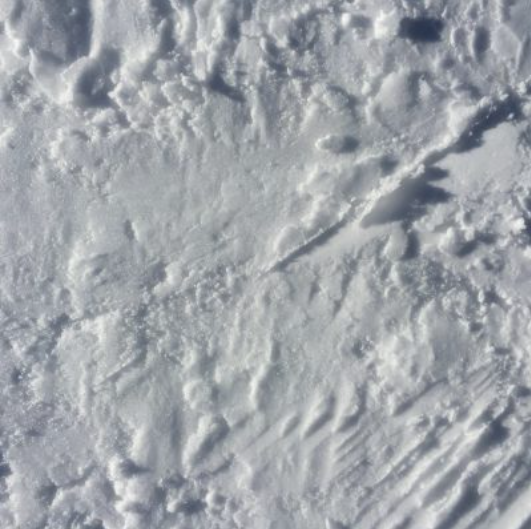
\includegraphics[width=\textwidth]{../Code/Textures/2.png}
        \caption{Texture 2}
        \label{fig:texture-2}
    \end{subfigure}
    \hfill % this will add space between the subfigures
    \begin{subfigure}[b]{0.32\textwidth}
        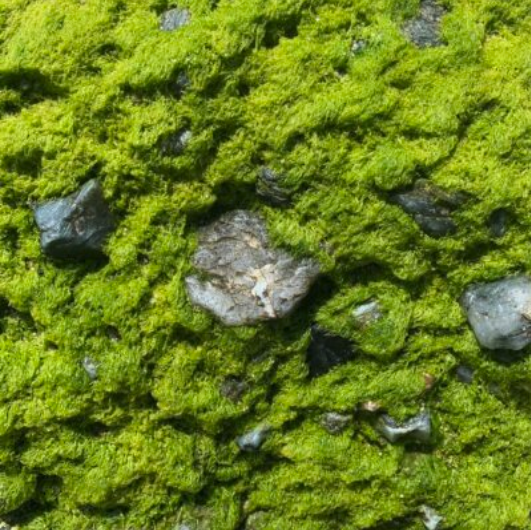
\includegraphics[width=\textwidth]{../Code/Textures/9.png}
        \caption{Texture 9}
        \label{fig:texture-9}
    \end{subfigure}
    \hfill % this will add space between the subfigures
    \begin{subfigure}[b]{0.32\textwidth}
        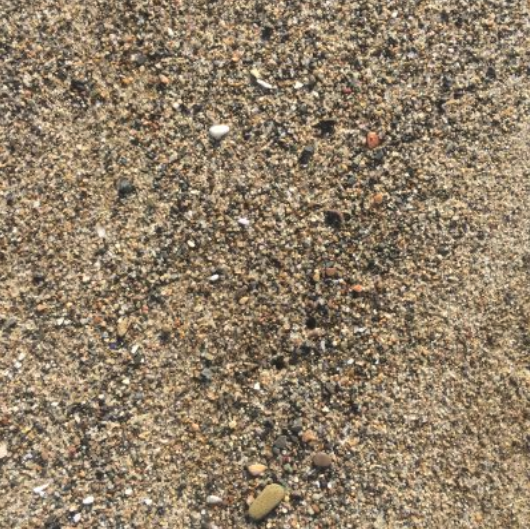
\includegraphics[width=\textwidth]{../Code/Textures/12.png}
        \caption{Texture 12}
        \label{fig:texture-12}
    \end{subfigure}
    \caption{Texture: provided in the class}
    \label{fig:texture-class}
\end{figure}

For the MNIST digits, we load the MNIST dataset ($28 \times 28$ handwritten digits)\footnote{Downloaded from \url{https://git-disl.github.io/GTDLBench/datasets/mnist_datasets/}}, including 60000 training images and 10000 testing images. 
We randomly select $20 \times 20$ images from the training set as the sample texture of size $560 \times 560$, shown in Figure~\ref{fig:texture-mnist}.

\begin{figure}[htbp!]
    \centering
    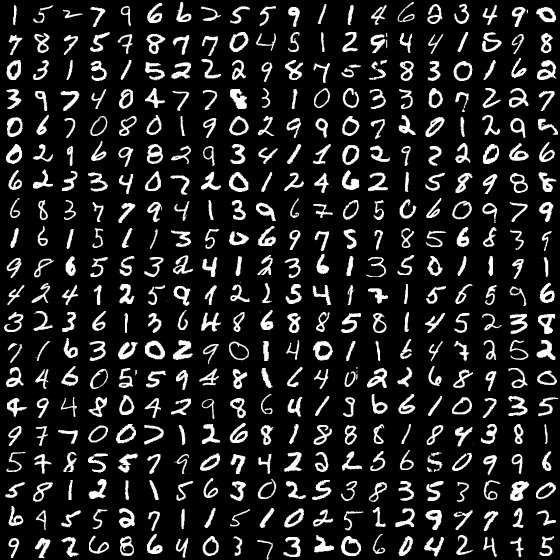
\includegraphics[width=0.5\textwidth]{../Code/Textures/mnist.png}
    \caption{Texture: MNIST digits}
    \label{fig:texture-mnist}
\end{figure}

For the galaxy picture, we load the galaxy picture ($800 \times 585$), shown in Figure~\ref{fig:texture-galaxy}.
\begin{figure}[htbp!]
    \centering
    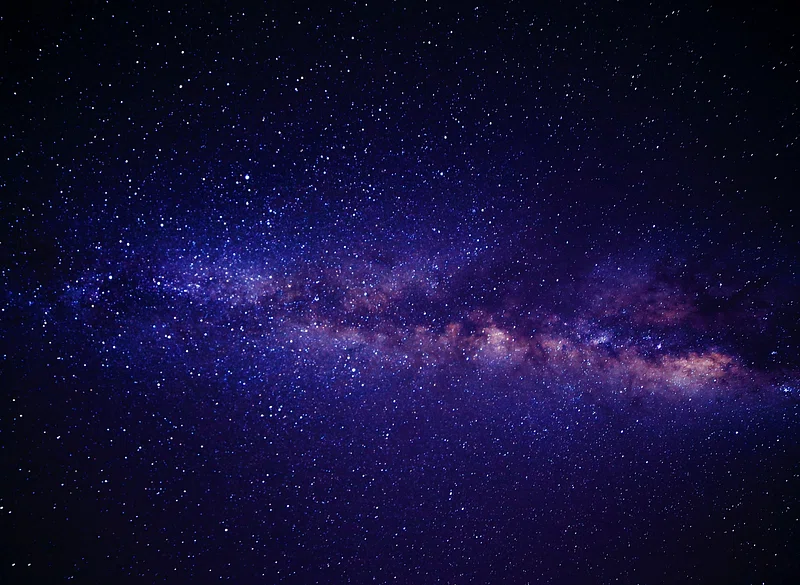
\includegraphics[width=0.5\textwidth]{../Code/Textures/galaxy.png}
    \caption{Texture: galaxy picture}
    \label{fig:texture-galaxy}
\end{figure}

\subsection{Non-parametric Texture Synthesis}

The algorithm proposed by Efros \& Leung (1999), Algorithm~\ref{alg:texture-synthesis}, synthesizes texture by modeling the image as a Markov Random Field (MRF) where each pixel's value is dependent only on the values in its immediate neighborhood. 
The texture synthesis process grows the new image pixel by pixel from an initial seed based on this model. Here are some important features about the algorithm:
\begin{itemize}
  \item {Non-parametric approach:} The algorithm does not build an explicit model but estimates pixel distributions dynamically from the sample image.
  \item {Control over randomness:} The size of the neighborhood window can be adjusted to control the randomness of the texture, affecting how structured or stochastic the synthesized texture appears.
  \item {Efficiency:} A variation of the k Nearest Neighbors technique is employed to find matching neighborhoods quickly.
  \item {Local structure preservation:} Emphasis on maintaining the local structure of the texture to ensure visual continuity and realism in the synthesized image.
\end{itemize}

\begin{algorithm}
    \caption{Texture Synthesis by Non-parametric Sampling}\label{alg:texture-synthesis}
    \begin{algorithmic}[1]
    
    \State Initialize with a small seed taken randomly from the sample image $I_{\text{smp}}$.
    
    \While{there are unsynthesized pixels in the image $I$}
        \State Select an unsynthesized pixel $p$ in $I$.
        \State Define the neighborhood $N(p)$ of $p$ as a square window centered at $p$.
        
        \State Find all neighborhoods in $I_{\text{smp}}$ that are similar to $N(p)$ using a perceptual distance metric $d_{\text{perc}}$.
        \State Construct a histogram of pixel values from these similar neighborhoods to approximate the conditional probability distribution $P(p|N(p))$.
        \State Sample from this distribution to set the value of $p$.
    \EndWhile
    
    \end{algorithmic}
\end{algorithm}

\subsection{Parallelization}

To speed up the texture synthesis process, we parallelize the algorithm by dividing the image into blocks and synthesizing each block independently, given that the processing of each pixel (and its surrounding window) is somewhat independent.
We use the Python \texttt{multiprocessing} library to create a pool of worker processes that can work on different blocks concurrently:
\begin{itemize}
    \item {Split the work:} Distribute the processing of each pixel to different CPU cores. This can be done by creating a list of tasks where each task contains the information needed to process a pixel.
    \item {Process pool:} Use a multiprocessing pool to process these tasks concurrently.
    \item {Result collection:} Collect the results from each task and update the main data structures accordingly.
\end{itemize}
With this parallelization strategy, we can achieve a significant speedup (depending on hardware, around $8\times$) in the texture synthesis process.

\section{Results}

Here we present the results of applying the non-parametric texture synthesis method to the textures described in the previous section.

\begin{figure}[htbp!]
    \centering
    \begin{subfigure}[b]{0.49\textwidth}
        \centering
        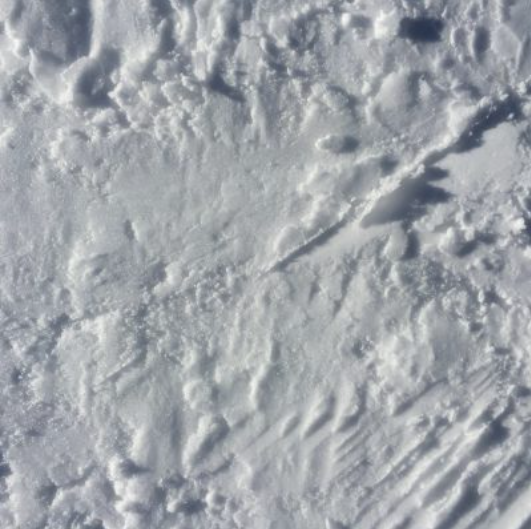
\includegraphics[width=0.5\textwidth]{../Code/Textures/2.png}
        \caption{Texture 2}
        \label{fig:original-2}
    \end{subfigure}
    \hfill % this will add space between the subfigures
    \begin{subfigure}[b]{0.49\textwidth}
        \centering
        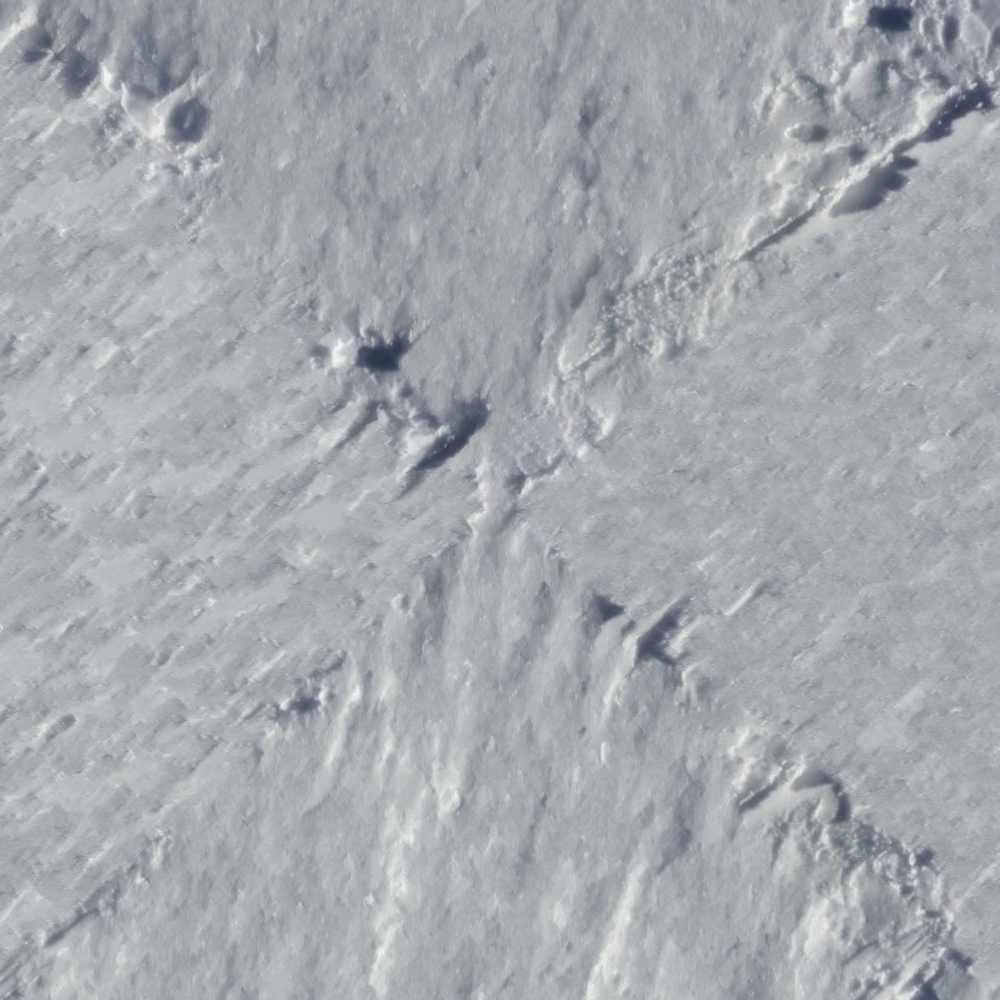
\includegraphics[width=\textwidth]{../Result/2.png}
        \caption{Synthesized Picture 2}
        \label{fig:synthesized-2}
    \end{subfigure}
    \caption{Synthesis of Texture 2}
    \label{fig:synthesis-2}
\end{figure}

\begin{figure}[htbp!]
    \centering
    \begin{subfigure}[b]{0.49\textwidth}
        \centering
        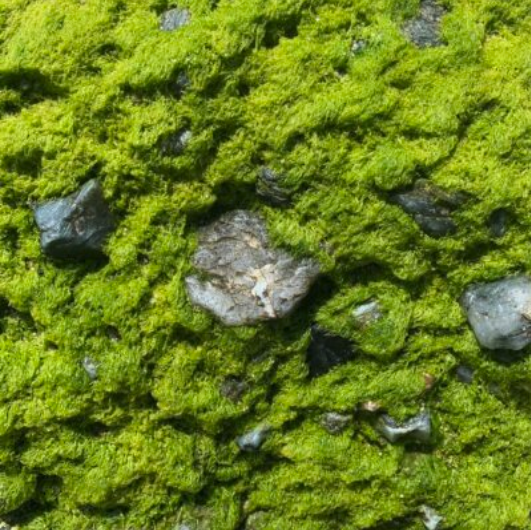
\includegraphics[width=0.5\textwidth]{../Code/Textures/9.png}
        \caption{Texture 9}
        \label{fig:original-9}
    \end{subfigure}
    \hfill % this will add space between the subfigures
    \begin{subfigure}[b]{0.49\textwidth}
        \centering
        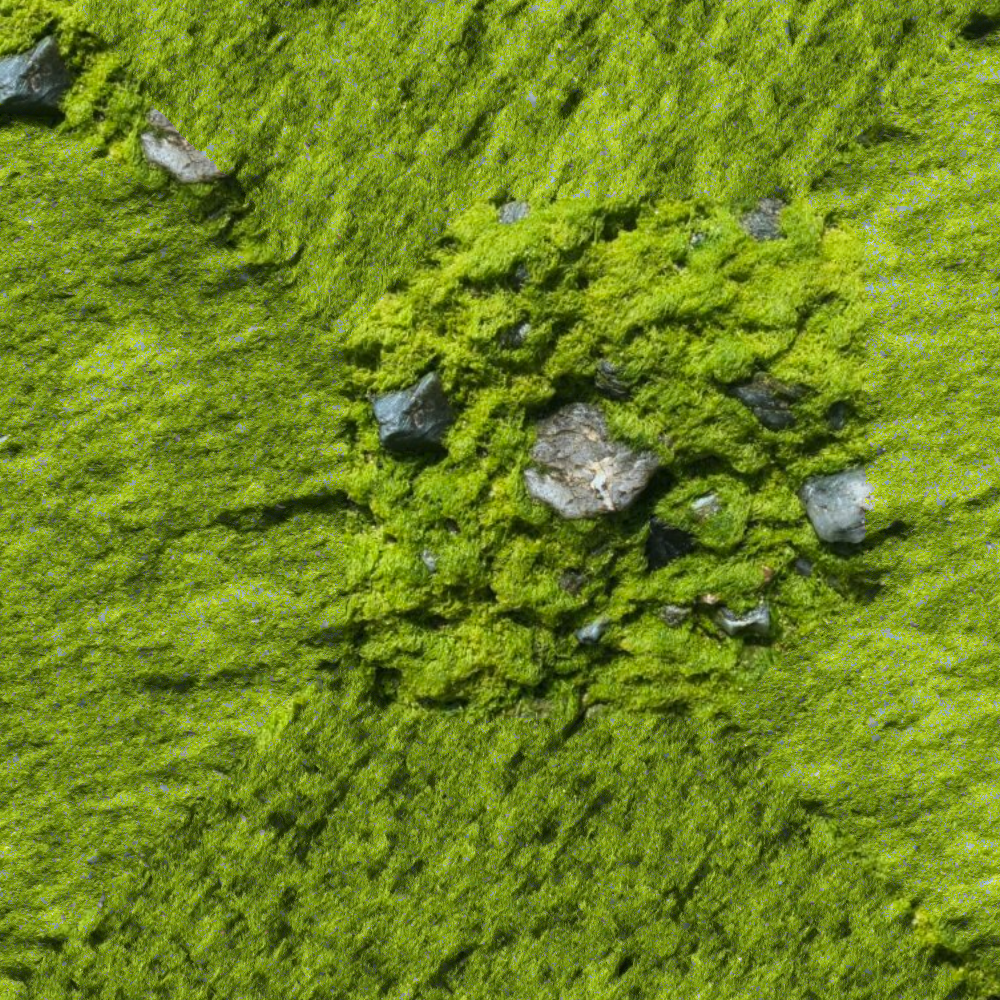
\includegraphics[width=\textwidth]{../Result/9.png}
        \caption{Synthesized Picture 9}
        \label{fig:synthesized-9}
    \end{subfigure}
    \caption{Synthesis of Texture 9}
    \label{fig:synthesis-9}
\end{figure}

\begin{figure}[htbp!]
    \centering
    \begin{subfigure}[b]{0.49\textwidth}
        \centering
        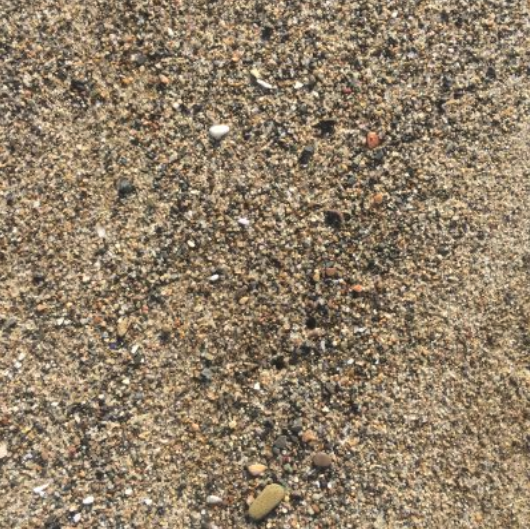
\includegraphics[width=0.5\textwidth]{../Code/Textures/12.png}
        \caption{Texture 12}
        \label{fig:original-12}
    \end{subfigure}
    \hfill % this will add space between the subfigures
    \begin{subfigure}[b]{0.49\textwidth}
        \centering
        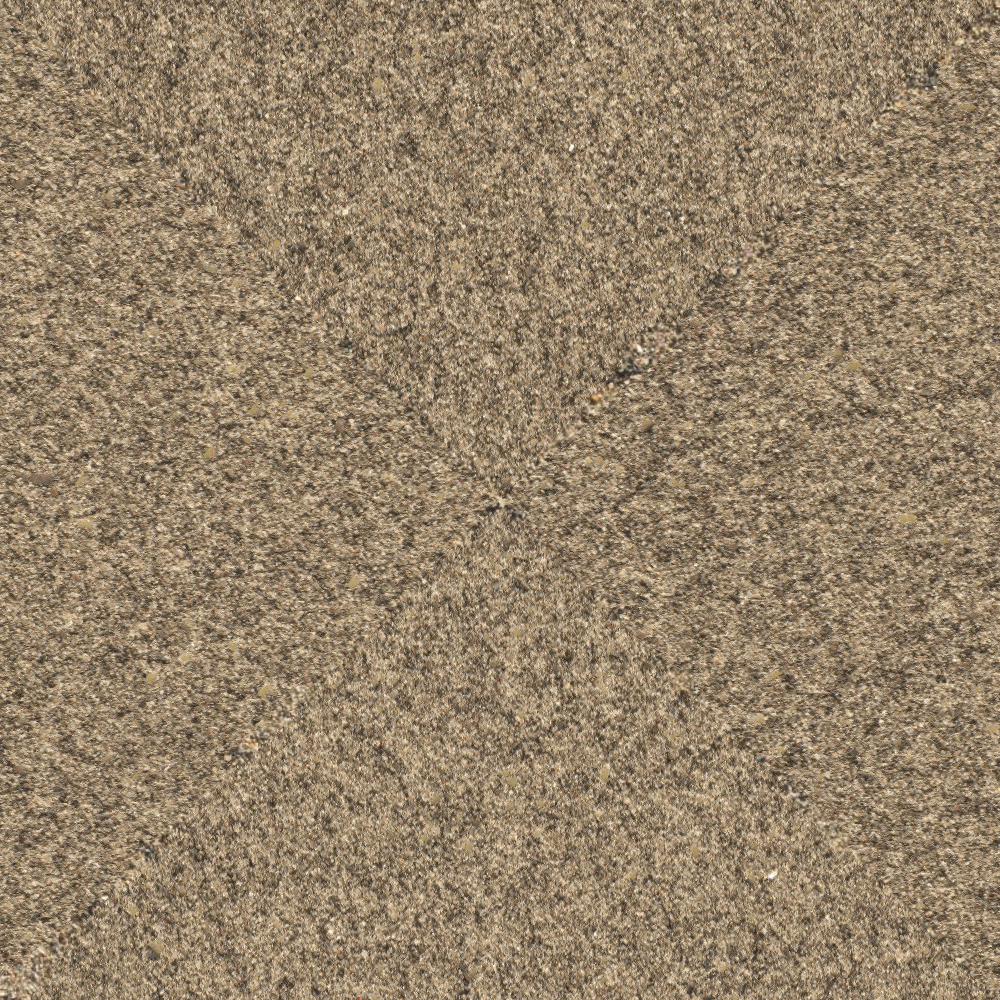
\includegraphics[width=\textwidth]{../Result/12.png}
        \caption{Synthesized Picture 12}
        \label{fig:synthesized-12}
    \end{subfigure}
    \caption{Synthesis of Texture 12}
    \label{fig:synthesis-12}
\end{figure}

\begin{figure}[htbp!]
    \centering
    \begin{subfigure}[b]{0.49\textwidth}
        \centering
        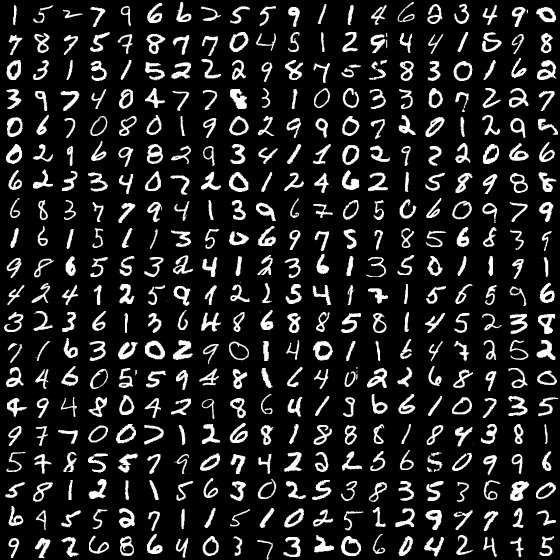
\includegraphics[width=0.5\textwidth]{../Code/Textures/mnist.png}
        \caption{MNIST Digits}
        \label{fig:original-mnist}
    \end{subfigure}
    \hfill % this will add space between the subfigures
    \begin{subfigure}[b]{0.49\textwidth}
        \centering
        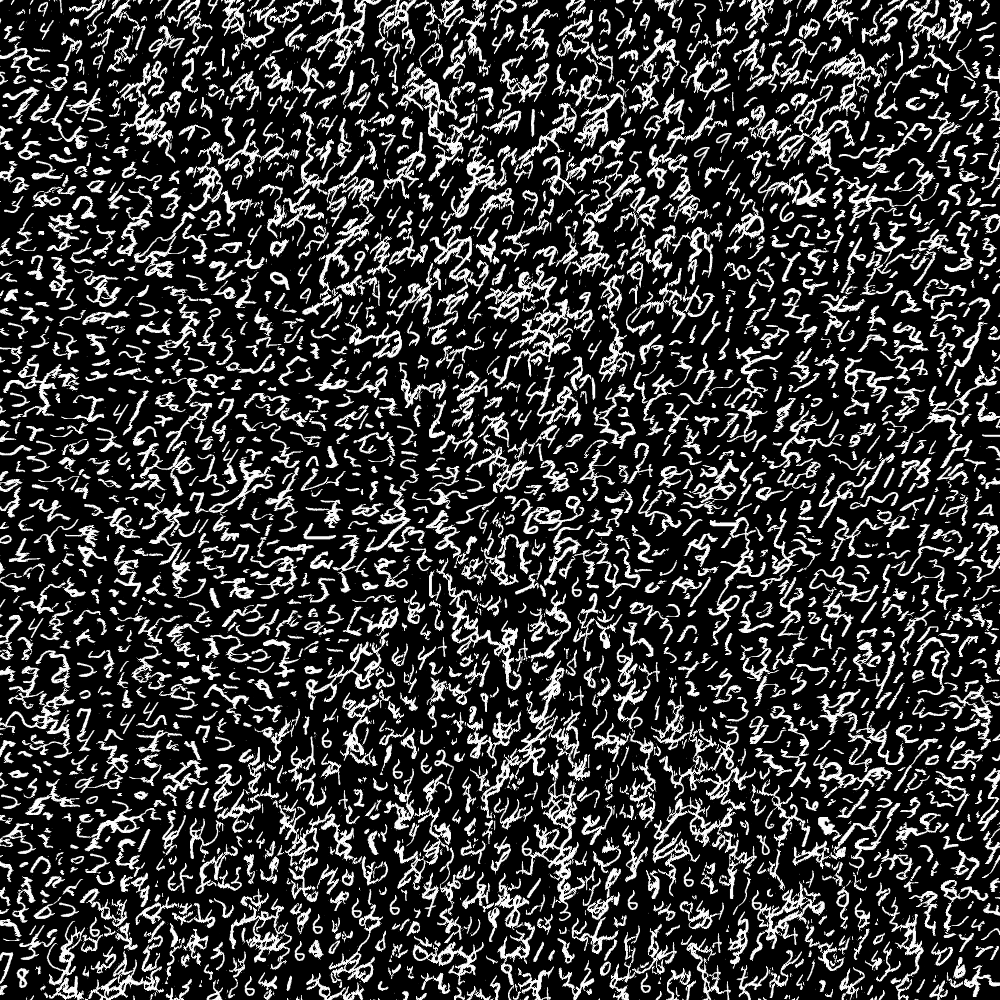
\includegraphics[width=\textwidth]{../Result/mnist.png}
        \caption{Synthesized MNIST Digits}
        \label{fig:synthesized-mnist}
    \end{subfigure}
    \caption{Synthesis of MNIST Digits}
    \label{fig:synthesis-mnist}
\end{figure}

\begin{figure}[htbp!]
    \centering
    \begin{subfigure}[b]{0.49\textwidth}
        \centering
        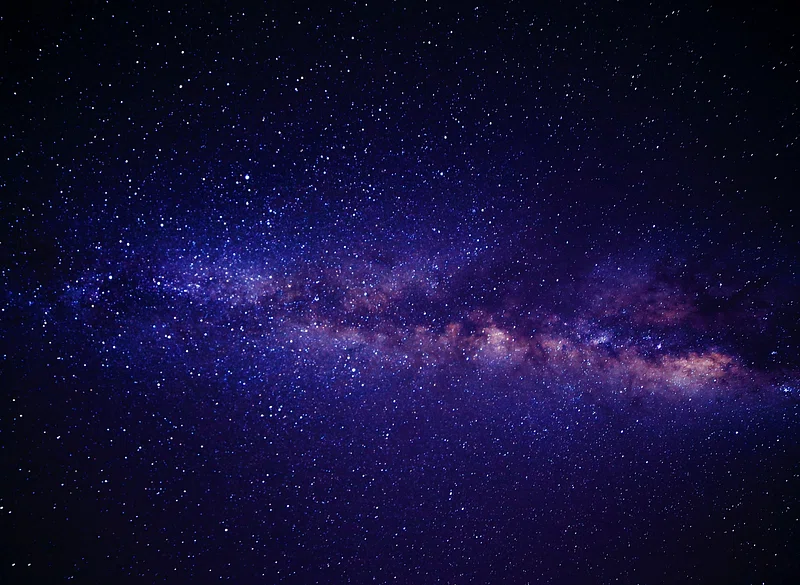
\includegraphics[width=0.6\textwidth]{../Code/Textures/galaxy.png}
        \caption{Galaxy Picture}
        \label{fig:original-galaxy}
    \end{subfigure}
    \hfill % this will add space between the subfigures
    \begin{subfigure}[b]{0.49\textwidth}
        \centering
        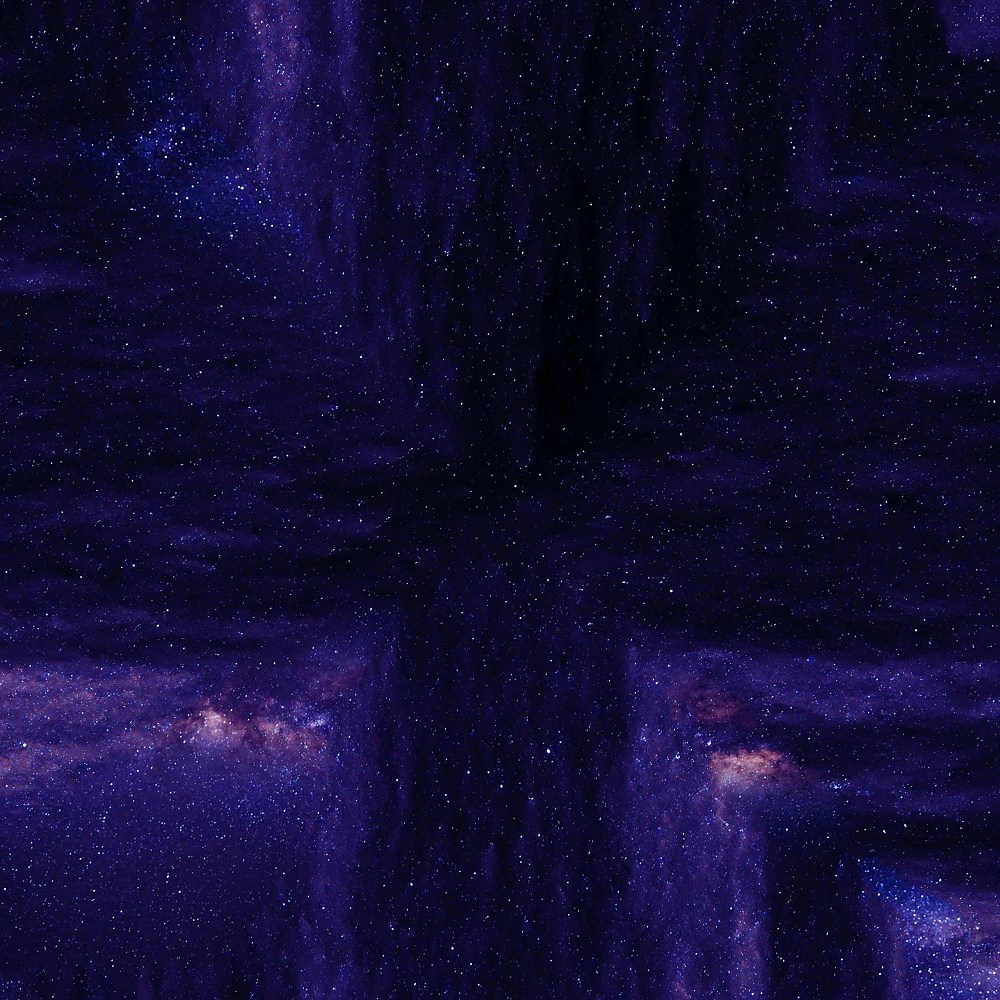
\includegraphics[width=\textwidth]{../Result/galaxy.png}
        \caption{Synthesized Galaxy Picture}
        \label{fig:synthesized-galaxy}
    \end{subfigure}
    \caption{Synthesis of Galaxy Picture}
    \label{fig:synthesis-galaxy}
\end{figure}



\end{document}
